\documentclass[11pt]{article}
\usepackage[utf8]{inputenc}
\usepackage[french]{babel}
\usepackage{graphicx}
\graphicspath{{./img/}}
\usepackage[left=3cm,right=3cm,top=2.5cm,bottom=2cm]{geometry}
\usepackage{url}
\usepackage{fancyhdr}
\pagestyle{fancy}
\fancyhead[L]{Projet S6}
\fancyhead[R]{Rapport de projet}

\fancyfoot[L]{Groupe 15528}
\fancyfoot[R]{Année 2021-2022}
\renewcommand\footrulewidth{0.5pt}

\usepackage{amsmath, amssymb}
\usepackage{tikz}
\usetikzlibrary{arrows,automata,shapes}

\begin{document}
\begin{figure}[h]
    \centering
    
\includegraphics[scale=0.55]{Logo_ENSEIRB-MATMECA-Bordeaux_INP.svg.png}
\end{figure}
\begin{center}
    

\Large Rapport de projet - Semestre 6 - Groupe 15528 \\
\vspace{0.5cm}
mai 2022
\vspace{2cm}
\begin{figure}[h]
\begin{tikzpicture}[scale=1.3]
\draw (0,0) -- (12,0);  
\end{tikzpicture}
\end{figure}\\
\vspace{1cm}
\textbf{\Huge Robot Programming}
\vspace{1cm}
\begin{figure}[h]
\begin{tikzpicture}[scale=1.3]
\draw (0,0) -- (12,0);  
\end{tikzpicture}
\end{figure}\\
\vspace{0.5cm}
Filière Informatique - ENSEIRB-MATMECA
\end{center}
\begin{flushleft}
Auteurs:\\
KHIARI Skander\\
KABBOU Meryem\\
MEDGHALI Majid \\
OUALI Mohammed \\
\vspace{0.5cm}
Encadrants:\\
M.MORANDAT Floréal\\
M.RENAULT David\\
\end{flushleft}

\newpage
\tableofcontents
\newpage



\section{Introduction }


\subsection{Contexte et présentation}
Ce projet s’est déroulé dans le cadre d’une évaluation pour le semestre 6.\\
Le sujet repose sur un petit robot chargé de ramasser des étoiles disséminées sur une grille colorée. L’attendu principal est d’impl\'ementer des fonctions qui permettent d'atteindre des objectifs sur des puzzles diff\'erents et d'afficher le trajet d'un robot lors de sa recherche. 


\subsection{Organisation et outils de travail}
Pour pouvoir d\'evelopper un programme fonctionnel dans le temps imparti, nous
avons \`a chaque instant, attribu\'e \`a un membre de groupe une t\^ache pr\`ecise. et pour l'\'echange des fichiers, on a utilisé un dépôt git. Cet outil nous permet par ailleurs en cas de probl\`eme avec la derni\`ere version
de revenir \`a la précédente. \\
LaTeX permet une mise en page claire et une facilit\'e d'\'ecriture de documents
scientifiques. Nous avons ainsi choisi de l’utiliser pour la r\'edaction de notre
rapport.

\section{Problématique}
%\subsection{Création du monde et des contextes}
\subsection{Description du puzzle}
Un puzzle est un objet dont les champs représentent des informations utiles sur le puzzle : id, title, robotRow, robotCol, robotDir, subs et board ces champs sont donnés par le sujet et on a ajouté un champ \textbf{stars} qui correspond au nombre des étoiles du puzzle. Pour pouvoir récupérer les informations d'un puzzle, on a implémenté des fonctions getPuzzleFrmId et getPuzzleFrmName qui nous permettent de récupérer un puzzle à partir de son nom ou son id.


\subsection{Récupération du puzzle et de la solution}
L'utilisateur peut entrer un puzzle et une solution de son choix à partir de la ligne de commande, deux cas sont possibles :
\begin{itemize}
    \item Soit l'utilisateur fait entrer, dans la ligne de commande, le nom d'un puzzle déjà définit dans le fichier \texttt{puzzles.js} et puis un fichier\textbf{.json} contenant la solution dans un champ sol d'un objet. Comme cela on aura juste à récupérer le puzzle choisi à l'aide de la fonction getPuzzleFrmName mentionnée dans la partie ci-dessus.
    \item Soit la solution et le puzzle sont donnés dans un fichier\textbf{.json}, passé en ligne de commande, qui contient un objet avec deux champs : sol pour la solution et puzzle pour le puzzle.\\ 
    La récupération des éléments d'un fichier \textbf{Json} a été faite à l'aide de \textbf{readFileSync()}, du module \textbf{fs} qui permet de lire le fichier et renvoyer son contenu, et de la fonction \textbf{Json.parse}, qui construit l'objet décrit par la chaîne de caractère passée en paramètre.
\end{itemize}
\subsection{Vérification de la solution et du puzzle }
nous avons implémenté plusieurs fonctions pour vérifier les erreurs statiques, c'est-à-dire si le puzzle et la solution sont valides. On vérifie la validité de la solution à partir de sa forme donnée par le champ \texttt{subs} du puzzle et la validité du puzzle à partir de sa forme générale.
\subsection{Implémentation d'un interpr\'eteur}
Après avoir récupéré le puzzle et la solution, nous devions appliquer cette dernière sur le puzzle en parcourant le programme de la solution et en appliquant chaque instruction sur le puzzle dans le cas ou le prédicat "c'est-à-dire la couleur de la case du puzzle" est vérifié, sinon on passe à l'instruction suivante si elle existe.
\subsection{Vérification de la fin d'exécution }
Le contrôle des itérations de la boucle principale nécessite de coder la fonction gameOver qui nous permet à la fin de chaque itération de savoir si la partie est terminée ou non. Cette fonction traite toutes les erreurs dynamiques possibles et vérifie si le robot a atteint son objectif qui est la collection de toutes les étoiles présentes dans le puzzle, d'où la nécessité d'ajouter dans le puzzle le champ \textbf{stars} représentant le nombre des étoiles. \\
Les erreurs dynamiques traitées pour savoir la fin de la partie sont les suivantes : si le robot sort de la trajectoire ou sort carrément du puzzle donné, si le robot arrive à gagner toutes les étoiles du puzzle ou si on a une boucle infinie qu'on définit par un nombre d'itérations supérieur ou égal à 500.


\section{Cadre du travail}
\subsection{Graphe de dépendance}

\begin{figure}[h]
    \centering
    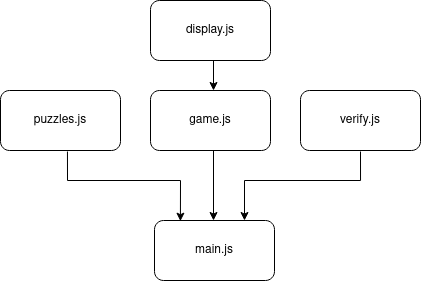
\includegraphics{Untitled Diagram.drawio(1).png}
    \caption{Diagramme de dépendance }
    \label{fig:Diagramme}
\end{figure}
Le diagramme ci-dessus \ref{fig:Diagramme} fait état des dépendances des fichiers de notre code.\\


Le fichier \texttt{main.js} contient la boucle principale du projet, qui récupère le puzzle et la solution et l'exécuté sur ce dernier.\\
Nous avons choisi de faire des fichiers séparés pour chaque module donc on a fait un fichier \texttt{display.js} pour l'affichage du puzzle, \texttt{verify.js}  pour vérifier la solution et le puzzle, \texttt{game.js} qui contient les fonctions utiles pour exécuter un programme sur un puzzle et \texttt{puzzles} qui contient des exemples de puzzles avec leurs solutions (utiles pour les tests).\\ 

\subsection{Architecture des fichiers et détails techniques}
Les fichiers dans le dépôt sont organisés de la manière suivante :\\
\begin{center}
    
    \begin{verbatim}
        /              -- la racine du répertoire du projet
        Makefile       -- Makefile global
        README.md      -- fichier qui contient les instructions d’exécution
        /src           -- fichiers sources et tests(.js)
        /public        -- fichiers Web
        /rapport       -- Rapport du projet (.tex/pdf)
    \end{verbatim}
        
\end{center}

Le fichier \texttt{Makefile} fournit :
\begin{itemize}
    \item \textbf{une règle \texttt{gen}} qui génère la page web avec parcel .
    \item \textbf{une règle \texttt{test}} qui exècute les tests.
\end{itemize}

\section{Mécanisme du jeu}
\subsection{Implémentation du programme et les instructions }
Pour qu'un robot résout un puzzle, il doit exécuter un programme sur un puzzle, ce programme est implémenté sous forme d'un tableau de fonctions de 1 à N. Chaque fonction contient des instructions constituées de deux champs \texttt{['ACTION', 'PRÉDICAT']}, l'action correspond soit au mouvement du robot, soit \`a l'appel d'une autre fonction et le prédicat correspond à la couleur nécessaire pour appliquer le premier champ.\\

Pour pouvoir exécuter une instruction, nous avons implémenté la fonction\\ \texttt{executeInstOnPuzzle} qui étant donné un couplet \texttt{['ACTION', 'PRÉDICAT']} et un context C\footnote{le contexte est objet défini comme suit :\\context = \{"puzzle" :puzzle,"prog" :prog,"stack" :[[0,0]],"pc" :[0,0],"num" :0, "error" :'NONE'\}; } applique l'action de cette dernière si le prédicat est vérifié. Si oui, on appelle la fonction \texttt{action} qui à son
tour appelle la fonction dédiée à l'instruction qui lui est passée en paramètre. 
\subsection{Implémentation de la boucle principale}
Après la récupération du puzzle et d'un programme, il fallait bien vérifier qu'ils sont valides. En effet, deux fonctions \texttt{verifyPuzzle} et \texttt{verifyProgram} assurent que le puzzle et de programme sont utilisables.\\
Après la vérification et pour exécuter le programme sur le puzzle, on a décidé d'implémenter une boucle de jeu à l'aide de la fonction \texttt{setInterval} qui déclenche répétitivement la même action à intervalles réguliers, la boucle de jeu appel répétitivement une fonction \texttt{moveRobot} qui est une fonction d'ordre supérieur qui prend en paramètres le contexte et une fonction d'affichage pour visualiser les résultats, le contexte qui décrit l'état actuel du jeu sera changé après chaque itération ou bien après chaque exécution de la fonction \texttt{moveRobot}.\\
En plus, après chaque itération, on vérifie la fin de l'exécution à l'aide de la fonction \texttt{gameOver}.
\begin{figure}[h!]
    \centering
    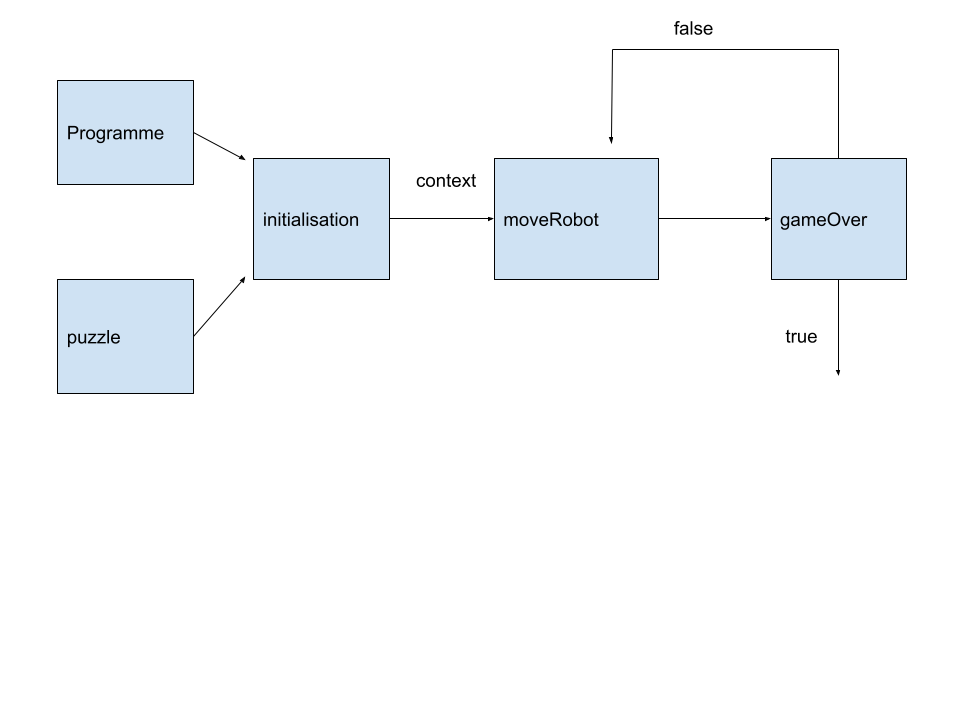
\includegraphics[scale=0.3]{dessin.png}
    \caption{La représentation de la boucle principale}
\end{figure}

\subsection{Visualisateur }
Pour visualiser correctement l'exécution de notre programme, on a eu l'idée d'implémenter un visualiseur en mode terminal qui affiche le puzzle et le robot a chaque itération. En effet, une fonction \texttt{display} dans le fichier.
\begin{figure}[h!]
\begin{center}
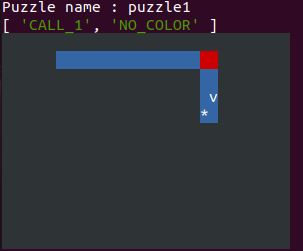
\includegraphics[scale=0.6]{puzzle2.png} \quad
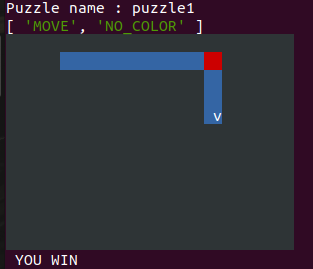
\includegraphics[scale=0.6]{puzzle1.png}
\caption{L'affichage de l'évolution du robot en mode terminal}
\end{center}
\end{figure}

\texttt{display.js}. En plus de ça une fonction \texttt{term} qui sert à afficher le puzzle en plus de résultat d'exécution et le message d'erreur.\\
Une partie de sujet propose de créer une page web pour visualiser l'exécution de programme sur les puzzles. sur notre interface, on a implémenté un ensemble de puzzles et l'utilisateur doit
insérer les instructions et les prédicats nécessaires pour gagner la partie.

\begin{figure}[h]
    \centering
    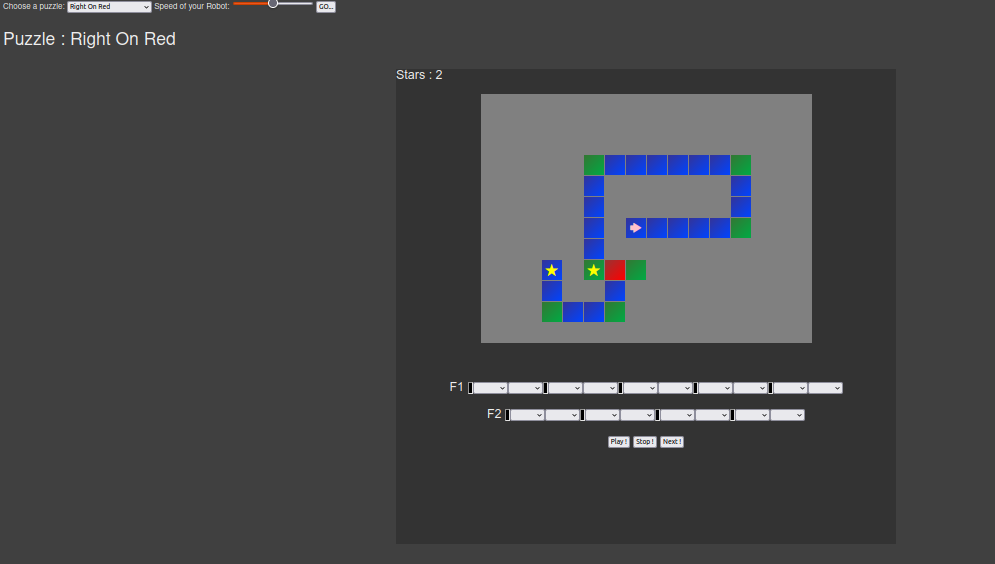
\includegraphics[scale=0.5]{html.png}
    \caption{La représentation en mode HTML}
\end{figure}



\section{Problèmes intéressants rencontrés et solutions algorithmiques}
\subsection{Utilisation du context et récupération des erreurs}

Pendant le déroulement du projet, nous nous sommes trouvés avec des fonctions dont les paramètres sont nombreux. D'où l'idée de créer une structure \textbf{context} qui regroupe les éléments suivants  :"puzzle" correspondant au puzzle concerné, "prog" correspondant à la solution, "stack" correspondant à la pile, "num" correspond au nombre d'itérations de la boucle principale.\\

Pour tester si les erreurs dynamiques et statiques sont bien révélées par nos fonctions, nous avions besoin de récupérer le types d'erreur détecter pour chaque cas et le comparer avec l'erreur attendue. Pour récupérer le type d'erreur révélé, nous avons choisi d'ajouter un champ \textbf{error} où en met "NONE" au début et si une erreur est détectée on met dans ce champ le message d'erreur qui doit être affiché.  \\

\subsection{Implémentation de la pile d'appel}
Pendant l'exécution de la solution sur le robot, si la solution contient un appel de fonction, alors toutes les instructions suivant cet appel de fonction ne vont pas être exécutées.\\
Pour palier à ce problème, nous avons utilisé une pile où on stocke la variable \texttt{pc}=['\texttt{ID\_FONCTION}',  '\texttt{ID\_INSTRUCTION\_DANS\_LA\_FONCTION}'] représentant les indices d'une instruction. \\On commence par empiler la première instruction de la première fonction. Pour gérer cette pile, on a implémenté la fonction \texttt{step} qui met à jour la pile et retourne le nouveau pc à exécuter.\\ Plusieurs cas de figure peuvent se présenter :\\
\begin{itemize}
    \item 
Si l'instruction est une simple instruction (pas d'appel de fonction) \texttt{step} change le dernier pc stocké dans la pile par le pc suivant en incrémentant l'indice de l'instruction dans la fonction et renvoie ce nouveau PC\\
\item Si l'instruction est un CALL \texttt{step} empile le PC correspondant à la première instruction de la fonction appelée et  renvoie ce PC.\\
\item  Si l'instruction correspond à une instruction simple en fin de fonction, \texttt{step} dépile le dernier PC, et puis retourne le dernier PC restant dans la pile après l'avoir incrémenté.\\
\end{itemize}
On appelle cette fonction jusqu'à ce que la pile soit vide et aucune autre instruction à appliquer, dans ce cas, on retourne PC=[-1,-1].\\
\subsection{Affichage terminal}
À part l'affichage en mode HTML, nous avions besoin de vérifier si la solution donnée s'exécuté correctement sur le puzzle ou non, pour cela on a pensé à faire un autre affichage dans le terminal sous forme de plusieurs images successives du puzzle, de la position du robot après un déplacement et de l'instruction appliquée. L'affichage des images n'est rien d'autre qu'un affichage du champ \texttt{board} du puzzle en utilisant les références des couleurs lors de l'exécution.
\section{Description des tests du projet }
\subsection{Les tests du projet}
Les tests des fichiers move.test.js et puzzles.test.js ont été faites pour assurer la validité des fonctions programmées. On a donc testé toutes les fonctions et dans chaque fonction, ou on a couvert toutes les lignes, tout cela a été réalisé en utilisant la bibliothèque \textbf{jest} qui nous permet de calculer le taux de couverture et contr\^oler les tests.
\begin{figure}[h]
    \centering
    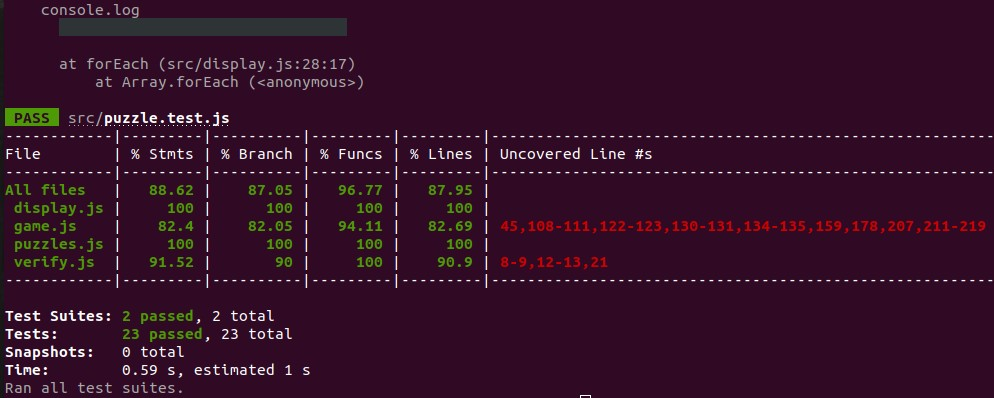
\includegraphics[scale=0.5]{ccovrage.jpg}
    \caption{Le taux de couverture des tests}
\end{figure}
\newpage
\subsection{Les tests d'exécutions}
On a testé tous les cas possibles qu'un utilisateur peut affronter lors de son expérience sur notre interface \textbf{HTML} les tests possibles sont : le robot sort de sa trajectoire, une boucle infinie, le robot ramasse toutes les étoiles et le cas de l'utilisateur ne donne pas de solution.
\begin{figure}[h!]
\begin{center}
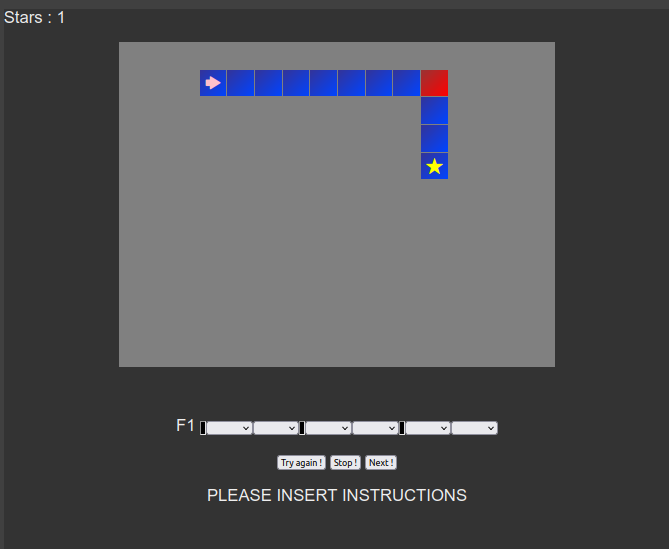
\includegraphics[scale=0.3]{html2.png} \quad
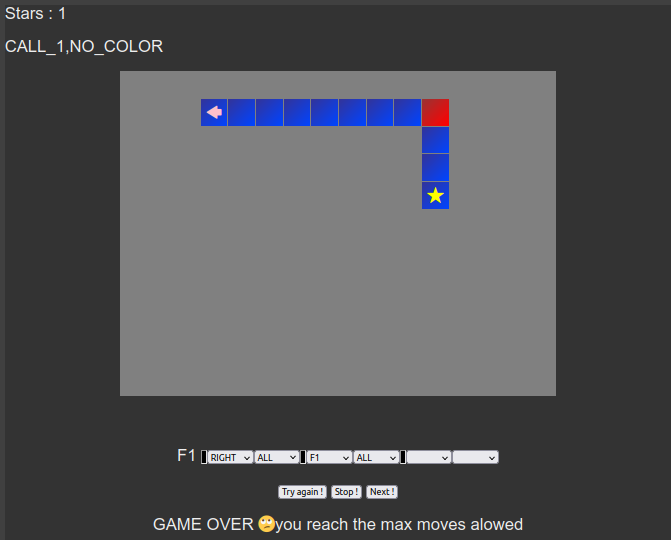
\includegraphics[scale=0.3]{html3.png}
\caption{Test d'exécution sans solution et test de boucle infinie}
\end{center}
\end{figure}
\begin{figure}[h!]
\begin{center}
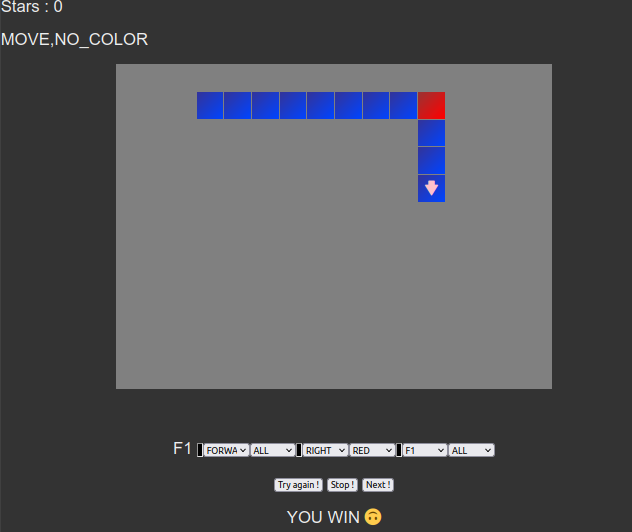
\includegraphics[scale=0.3]{html4.png} \quad
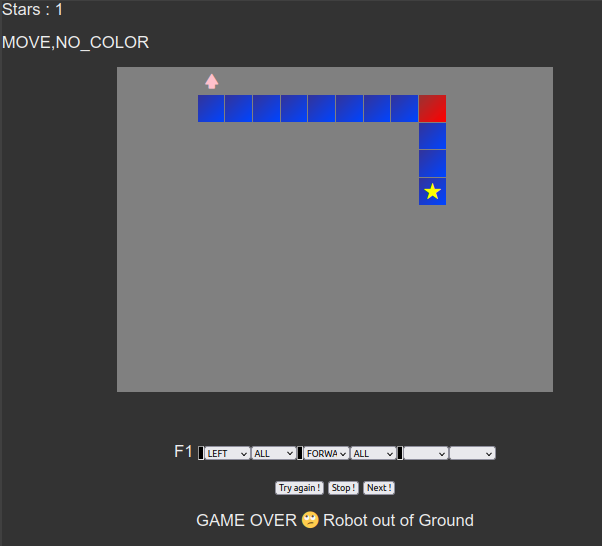
\includegraphics[scale=0.3]{html5.png}
\caption{Test d'exécution d'une solution correcte et d'un robot "Out of ground" }
\end{center}
\end{figure}
\begin{figure}[h!]
\begin{center}
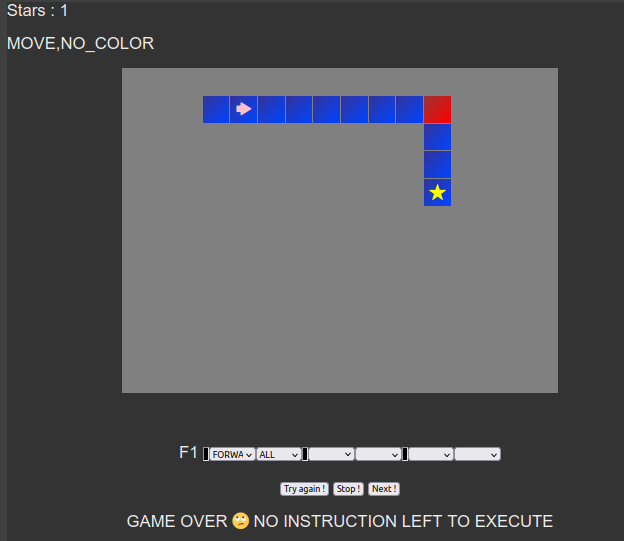
\includegraphics[scale=0.3]{no_instr.png} 
\caption{Test d'exécution d'une solution non complete }
\end{center}
\end{figure}


\newpage


\section{Discussion}
\subsection{Limites et améliorations possibles}
Plusieurs améliorations sont envisageables : Par exemple, une fonction qui prend en paramètre un puzzle et retourne un programme résolvant ce puzzle.\\ De plus, une extension du puzzle est possible en ajoutant d'autres éléments que les étoiles, ce qui permet de complexifier le puzzle.\\
\textbf{pureté et effets de bords}\\
Pour améliorer notre projet, on peut réécrire les fonctions programmées en les rendant des fonctions pures. Ainsi, on minimisera les effets de bords, on aura un code plus simple, plus flexible et facile à tester.\\

\subsection{Problèmes rencontrés}
Premièrement, nous avions une contrainte sur l'écriture du code mode HTML vu que c'est notre première expérience avec ce langage, et donc au début, on a perdu beaucoup de temps à faire des recherches sur internet afin de comprendre ce langage et pouvoir faire des améliorations pour faciliter l'utilisation de notre interface web. \\
Dans le cadre de la programmation fonctionnelle et en ce qui concerne la pureté du code, on a essayé d'écrire un code pur dans le maximum des fonctions, mais cela a été difficile à réaliser tout en gardant un code valide.\\
On a aussi trouvé des difficultés dans l'importation des fonctions d'un fichier vers un autre en utilisant les modules du \textbf{Ecmascript} vu qu'on le faisait avant avec les modules du \textbf{commonJS} qu'on a fait pendant les séances de TD.\\

\section{Conclusion}
Dans le cadre des projets de programmation, nous avons donc réalisé un pro-
gramme du jeu Robozzle. Ce projet a permis de mettre en œuvre les connais-
sances que nous avons acquis dans le cours de programmation fonctionnelle et de les améliorer. Nous avons été confrontés à de nombreux problèmes, mais nous avons pu
trouver des solutions alternatives pour les résoudre.\\
Le travail en groupe était enrichissant pour la confrontation d’idées et a été une bonne manière de progresser, à la fois sur le code et sur la manière d’appréhender et de résoudre les problèmes.


\end{document}
